\documentclass[aspectratio=169,compress,10pt]{beamer}
\usepackage[utf8]{inputenc}
\usepackage[T1]{fontenc}
\usepackage{lipsum, lmodern}
\usepackage{textcomp}
\usepackage{algorithm}
\usepackage{algorithmic}
\usetheme{Szeged} % or Median, or Metro, or PraterStreet, or Milano

\usecolortheme{spruce}

\author{Rafael Pérez-Torres \\ Selected Topics on Pattern Recognition}
\title{Swarm Intelligence \\ Particle Swarm Optimization}
\institute{Cinvestav Tamaulipas}
\date{\today}

\begin{document}
\frame{\maketitle}
\begin{frame}{Table of contents}
	\tableofcontents
\end{frame}

\section{Introduction}
\subsection{Artificial Intelligence}

% subsection ia (end)
\begin{frame}{Introduction}
% {\Large{} Why cross validation and resampling?} 
\begin{itemize}
	\item A major thrust in algorithmic development is the design of algorithmic models to solve increasingly complex problems.
	\item Enormous successes have been achieved through the modeling of biological and natural intelligence, resulting in so-called \emph{intelligent systems}.
	\item Together with logic, deductive reasoning, expert systems, case-based reasoning and symbolic machine learning systems, these intelligent algorithms form part of the field of Artificial Intelligence (AI).
\end{itemize}

\begin{block}{What is AI}
The study of how to make computers do things at which people are doing better
\end{block}

\end{frame}

\subsection{Computational Intelligence}
\begin{frame}{Introduction}
% {\Large{} Why cross-validation and resampling?} 
\begin{block}{What is computational intelligence (CI)}
The study of adaptive mechanisms to enable or facilitate intelligent behavior in complex and changing environments.
These mechanisms include those AI paradigms that exhibit an ability to learn or adapt to new situations, to generalize, abstract, discover and associate
\end{block}
\begin{itemize}
	\item (NN, Neural Networks)
	\item (EC, Evolutive Computing)
	\item (SI, Swarm Intelligence)
	\item (AIS, Artificial Immune Systems)
	\item (FS, Fuzzy Systems)
\end{itemize}
Each of the CI paradigms has its origins in biological systems.
\end{frame}

\subsection{Swarm Intelligence}
\begin{frame}{Swarm intelligence}
\begin{itemize}
	\item You and a group of friends are on a treasure finding mission. 
	\item You want that treasure, or at least some part of it.
	\item All who have taken part in the search will be rewarded: the person who found the treasure getting a higher reward; all others being rewarded based on distance from the treasure.
	\item Each one in the group has a metal detector and can communicate the strength of the signal and his current location to the nearest neighbors.
	\item What actions will you take? 
	\begin{itemize}
		\item Ignore your friends. If you find the treasure, it is all yours. However, if you do not find it first, you get nothing.
		\item Make use of the information from your neighboring friends, and move in the direction of your closest friend with the strongest signal.
		You increase your chances of finding the treasure, or at least maximizing your reward.
	\end{itemize}
\end{itemize}
\end{frame}

\begin{frame}{Swarm intelligence}
\begin{itemize}
	\item Swarm intelligence (SI) refers to the problem-solving behavior that emerges from the interaction of such agents.
	\item Computational swarm intelligence (CSI) refers to algorithmic models of such behavior.
	\item More formally, swarm intelligence is the property of a system whereby the collective behaviors of unsophisticated agents interacting locally with their environment cause coherent functional global patterns to emerge.
	Swarm intelligence has also been referred to as \emph{collective intelligence}.
\end{itemize}
\end{frame}

\section{Particle Swarm Optimization}
\begin{frame}{Particle Swarm Optimization, PSO}
\begin{itemize}
	\item The particle swarm optimization (PSO) algorithm is a population-based search algorithm based on the simulation of the social behavior of birds within a flock.
	\item Individuals in a particle swarm follow a very simple behavior: to emulate the success of neighboring individuals and their own successes.
	\item The collective behavior that emerges from this simple behavior is that of discovering optimal regions of a high dimensional search space.
	\item In analogy with evolutionary computation paradigms, a \emph{swarm} can be considered as a population and a \emph{particle} an individual.
\end{itemize}
\end{frame}

\begin{frame}{PSO}
\begin{itemize}
	\item The particles are \emph{flown} through a multidimensional search space, where the position of each particle is adjusted according to its own experience and that of its neighbors.
	\item Let $\mathbf{x}_i(t)$ denote the position of particle $i$ in the search space at time step $t$. The position of the particle is changed
by adding a velocity, $\mathbf{v}_i(t)$, to the current position
\begin{equation}
	\mathbf{x}_i(t+1) = \mathbf{x}_i + \mathbf{v}_i(t+1)
	\label{eq:velocidad-particula-generica}
\end{equation}
with $\mathbf{x}_i(0) \sim U(\mathbf{x}_\text{min},\mathbf{x}_\text{max}$).
	\item The velocity vector drives the optimization process, reflecting the experiential knowledge of the particle (\emph{cognitive component}) and socially exchanged information from the particle's neighborhood (\emph{social component}).
	\item Originally, two PSO algorithms have been developed which differ in the size of their neighborhoods: \emph{gbest} (global) and \emph{lbest} (local) PSO.
\end{itemize}
\end{frame}

\subsection{Global best PSO}
\begin{frame}{Global best PSO}
\begin{itemize}
	\item The neighborhood for each particle is the entire swarm (\emph{star} topology).
	\item In this case, the social information is the best position found by the swarm, $\mathbf{\hat{y}}(t)$.
	\item For \emph{gbest} PSO, the velocity of particle $i$ is calculated as:
	\begin{equation}
	v_{ij}(t+1) = v_{ij}(t) + c_1r_{1j}(t)[y_{ij}(t) - x_{ij}(t)] + c_2 r_{2j}(t)[\hat{y}_j(t) - x_{ij}(t)]
	\label{eq:velocidad-gbest}
	\end{equation}
	
	\item $v_{ij}(t)$ is the velocity of particle $i$ in dimension $j=1,\ldots,n_x$ at time step $t$, $x_{ij}(t)$ is the position of particle $i$ in dimension $j$ at time step $t$, $c_1$ and $c_2$ are positive acceleration constants used to scale the contribution of the cognitive and social components respectively, and $r_{1j}(t), r_{2j}(t) \sim U(0,1)$ are random values that introduce a stochastic element to the algorithm.
\end{itemize}
\end{frame}

\begin{frame}{Global best PSO II}
\begin{itemize}
	\item The personal best position, $\mathbf{y}_i$ , associated with particle $i$ is the best position the particle has visited since the first time step.
	\item Its best position in time $t+1$ is calculated as:
	\begin{equation}
\mathbf{y}_i(t+1) = \begin{cases}
               \mathbf{y}_i(t)	& \text{if } f(\mathbf{x}_i(t+1)) \geq f(\mathbf{y}_i(t))\\
               \mathbf{x}_i(t+1)	& \text{if } f(\mathbf{x}_i(t+1)) < f(\mathbf{y}_i(t))\\
           \end{cases}	
\end{equation}
where $f: \mathbb{R}^{n_x} \to \mathbb{R}$ is the fitness function.
\item The global best position, $\mathbf{\hat{y}}(t)$, in time step $t$ is calculated as:
$$
\mathbf{\hat{y}}(t) \in \left \{ \mathbf{y}_0(t), \ldots, \mathbf{y}_{n_s}(t) \right \} | | f(\mathbf{\hat{y}}(t)) = \text{min} \left \{ f(\mathbf{y}_0(t)),\ldots,f(\mathbf{y}_{n_s}(t)) \right \}
$$
where $n_s$ is the number of particles in the swarm.
\end{itemize}
\end{frame}


\begin{frame}{Global best PSO III}
\begin{algorithm}[H]
\scriptsize
\begin{algorithmic}[1] 
\STATE Crear e inicializar un enjambre de $n_x$ dimensiones
\REPEAT
	\FOR {cada partícula i = 1, $\ldots$, $n_s$}
		\STATE // Establecer la mejor posición personal
		\IF { $f(x_i) < f(y_i)$ }
			\STATE $y_i = x_i$
		\ENDIF
		\STATE // Establecer la mejor posición global 
		\IF {$f(y_i) < f(\hat{y})$}
			\STATE $\hat{y} = y_i$
		\ENDIF
	\ENDFOR
	\FOR {cada partícula i = 1, $\ldots$, $n_s$}
		\STATE Actualizar la velocidad utilizando \ref{eq:velocidad-gbest}
		\STATE Actualizar la posición utilizando la ecuación \ref{eq:velocidad-particula-generica}
	\ENDFOR
\UNTIL {se cumpla la condición de paro}
\end{algorithmic} 
\caption{PSO gbest} 
\label{alg:algoritmo-pso-gbest}
\end{algorithm}
\end{frame}

\begin{frame}{Global best PSO IV}
\begin{block}{\emph{gbest} algorithm behavior}
\centering
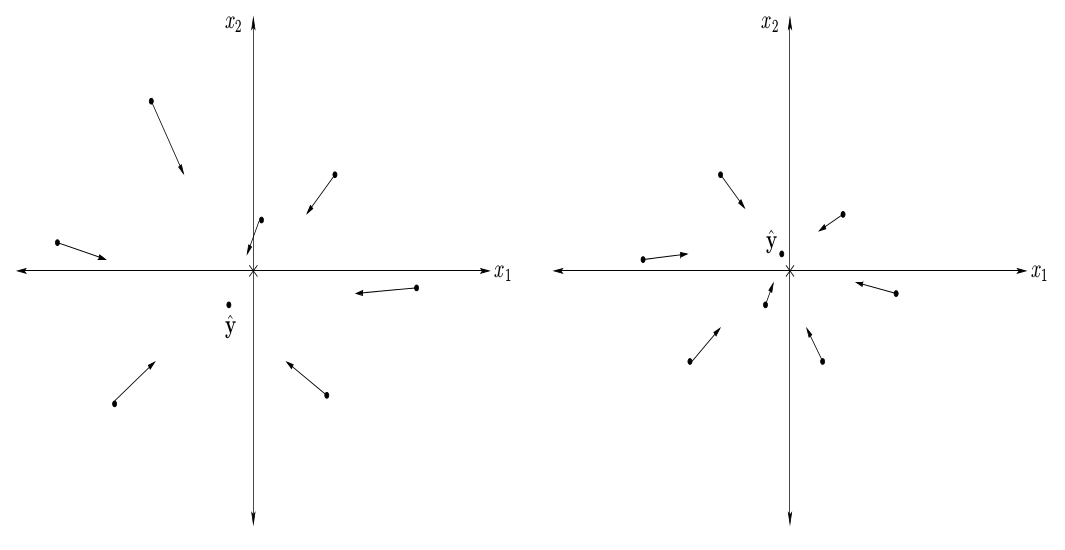
\includegraphics[scale=0.25]{../resources/gbest-behavior}
\end{block}
\end{frame}

\subsection{Local best PSO}
\begin{frame}{Local best PSO}
\begin{itemize}
	\item Uses a ring social network topology where smaller neighborhoods are defined for each particle.
	\item The social component reflects information exchanged within the neighborhood of the particle, reflecting local knowledge of the environment
	\item velocity is calculated as:
\begin{equation}
	v_{ij}(t+1)=v_{ij}(t) + c_1 r_{1j}[y_{ij}(t) - x_{ij}(t)] + c_2 r_{2j}(t) [\hat{y}_{ij}(t) - x_{ij}(t)]
	\label{eq:velocidad-lbest}
\end{equation}
where $\hat{y}_{ij}$ is the best position found in the neighborhood of particle $i$ in dimension $j$.
\end{itemize}
\end{frame}

\begin{frame}{Local best PSO II}
\begin{itemize}
	\item Then $\mathbf{\hat{y}}_i$ is the best position found in neighborhood $\mathcal{N}_i$ and is defined as:
$$
\mathbf{\hat{y}}_i (t+1) \in \left \{ \mathcal{N}_i | f( \mathbf{\hat{y}}_i (t+1) ) = \text{min} \left \{ f(x) \right \}, \forall \mathbf{x} \in \mathcal{N}_i \right \}
$$
\item Neighborhood $\mathcal{N}_i$ is defined as:
$$
\mathcal{N}_i = \left \{ y_{{i-n}_{\mathcal{N}_i}}(t), y_{i-n_{\mathcal{N}_i}+1 }(t), \ldots, y_{i-1}(t), y_{i+1}(t), \ldots, y_{i+n_{\mathcal{N}_i} }(t) \right \}
$$
\item Global best PSO is a special case of local best PSO with $n_{\mathcal{N}_i} = n_s$
\end{itemize}
\end{frame}

\begin{frame}{Local best PSO III}
\begin{algorithm}[H]
\scriptsize
\begin{algorithmic}[1] 
\STATE Crear e inicializar un enjambre de $n_x$ dimensiones
\REPEAT
	\FOR {cada partícula i = 1, $\ldots$, $n_s$}
		\STATE // Establecer la mejor posición personal
		\IF { $f(x_i) < f(y_i)$ }
			\STATE $y_i = x_i$
		\ENDIF
		\STATE // Establecer la mejor posición global 
		\IF {$f(y_i) < f(\hat{y})$}
			\STATE $\hat{y} = y_i$
		\ENDIF
	\ENDFOR
	\FOR {cada partícula i = 1, $\ldots$, $n_s$}
		\STATE Actualizar la velocidad utilizando \ref{eq:velocidad-lbest}
		\STATE Actualizar la posición utilizando la ecuación \ref{eq:velocidad-particula-generica}
	\ENDFOR
\UNTIL {se cumpla la condición de paro}
\end{algorithmic} 
\caption{Algoritmo PSO lbest} 
\label{alg:algoritmo-pso-lbest}
\end{algorithm}
\end{frame}

\begin{frame}{Local best PSO IV}
\begin{block}{\emph{lbest} algorithm behavior}
\centering
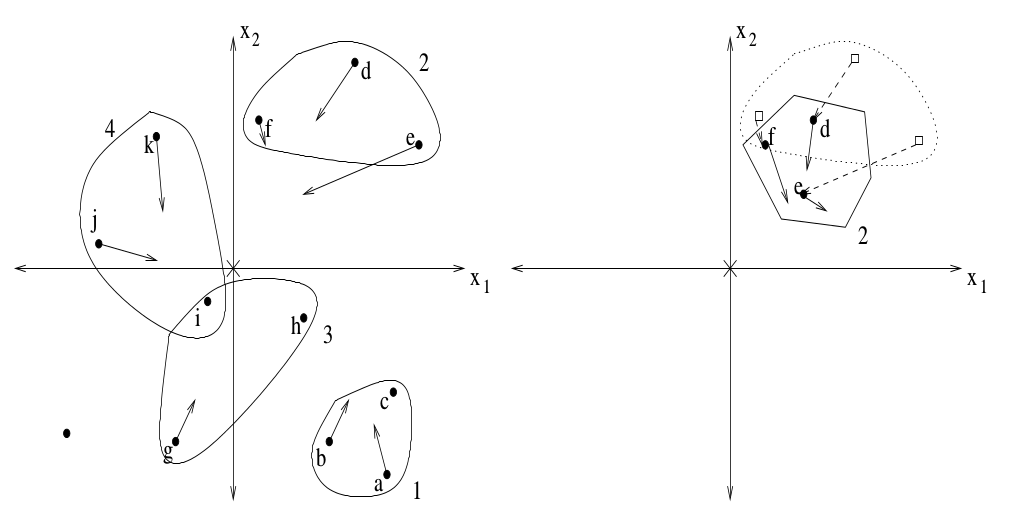
\includegraphics[scale=0.25]{../resources/lbest-behavior}
\end{block}
\end{frame}


\subsection{Stop criteria}
\begin{frame}{Stop criteria}
\begin{itemize}
	\item A maximum number of iterations.
	\item An acceptable solution is found: $f(x_i) \leq |f(x^*) - \epsilon |$.
	\item No improvement after a certain number of iterations.
	\item Swarm normalized radio is close to 0.
	\item Slope of objective function is approximately 0.
\end{itemize}
\end{frame}

\subsection{Global best vs Local best PSO}
\begin{frame}{Global vs local best PSO}
\begin{itemize}
	\item Due to larger particles connectivity, \emph{gbest} PSO converges faster, but it comes with the cost of less diversity than \emph{lbest} PSO.
	\item In this regard, \emph{lbest} PSO covers larger regions of search space becoming less sensible to local optimum.
	In general, neighborhood structures like star topology offer the best performance.
	\item Terminar cuando la pendiente de la función objetivoes aproximadamente 0.
\end{itemize}
\end{frame}


\subsection{Basic PSO parameters}
\begin{itemize}
	\item \textbf{Swarm size, $n_s$}: the more amount of particles, the more initial diversity and a larger region of search space can be covered.
	Also, it may improve convergence but also increase computational complexity.
	\item \textbf{Neighborhood size}: the smaller the neighborhood the smaller interaction and slower convergence; however it will improve quality of solutions.
	It is possible to start with small neighborhoods and then increase their size.
	\item \textbf{Iterations}: depending on scenario; a few iterations may produce premature search stop; many iterations migh cause unnecesary computations.
	\item \textbf{Acceleration coefficients}, $c_1$ y $c_2$: control the stochastic influence over cognitive and social components. 
	$c_1$ expresses how much confidence has the particle on itself, while  $c_2$ expresses the confidence the particle has in its neighbors.
\end{itemize}

\section{PSO variants}
\subsection{Variants}

\begin{frame}{PSO variants I}
\begin{block}{Velocity clamping}
To control the global exploration of particles, velocities
are clamped to stay within boundary constraints.
If a particle’s velocity in a dimension $d$ exceeds
a specified maximum velocity, the particle’s velocity is set to the maximum velocity.

This clamping is done jus after calculatin the new speed in the PSO algorithm.
\end{block}
    
\begin{block}{Inertia weight}
Is a mechanism to
control the exploration and exploitation abilities of the swarm, aimed at eliminating the need for velocity clamping.
Basically, $\omega$ controlls how much memory of
the previous flight direction will influence the new velocity.

In global PSO the velocity equation changes to
\begin{equation}
	v_{ij}(t+1) = \omega v_{ij}(t) + c_1r_{1j}(t)[y_{ij}(t) - x_{ij}(t)] + c_2 r_{2j}(t)[\hat{y}_j(t) - x_{ij}(t)]
	\label{eq:velocidad-peso-inercia}
\end{equation}
\end{block}

\end{frame}


\begin{frame}{PSO variants II}
\begin{block}{Constriction Coefficient}
An approach very similar to the inertia weight to balance the
exploration–exploitation trade-off, where the velocities are constricted by a constant $\mathcal{X}$, referred to as the constriction coefficient.

The velocity update equation changes to:
\begin{equation}
	v_{ij}(t+1) = \mathcal{X} [ v_{ij}(t) + \phi_1 (y_{ij}(t) - x_{ij}(t)) + \phi_2(\hat{y}_j(t) - x_{ij(t)})   ]
\end{equation}

where
$$
\mathcal{X} = \frac{2 \kappa}{| 2 - \phi - \sqrt{\phi ( \phi - 4)}  |}
$$
y $\phi = \phi_1 + \phi_2$, $\phi_1 = c_1 r_1$ y $\phi_2 = c_2 r_2$.
According to a formal analysis of eigenvalues of swarm dynamics,  $\phi \geq 4$ and $\kappa \in [0,1]$.
\end{block}
\end{frame}


\begin{frame}{PSO variants III}
\begin{block}{Synchronous versus Asynchronous Updates}
Original PSO algorithms update best positions isolated from particles position updates.
It is possible to perform the update of best positions after updating each particle, improving thee performance of \emph{lbest}.
\end{block}
\end{frame}

\begin{frame}{PSO variants IV}
\begin{block}{Velocity models}
Alternative velocity models differ in the components included in the velocity equation, and how best positions are determined.
\begin{itemize}
	\item \textbf{Cognition-only model}: exluced the social component from velocity equation.
	This resembles nostalgia since particles may return toward their previous best positions.
	\item \textbf{Social only model}: Excludes the cognitive component from the velocity equation.
	All particles are then attracted towards the best position of their neighborhood.
	\item \textbf{Selfless model}:
	Similar to social model, but the neighborhood best solution is only chosen from a particle's neighborhood.
	The particle itself is not allowed to become the neighborhood best.
\end{itemize}
\end{block}
\end{frame}

\section{Topologies} 
\begin{frame}{Topologies}
\begin{itemize}
	\item Social interaction guides PSO, and it is determined by the formation of overlapping neighborhoods.
	\item The information flow through a social network depends on:
	\begin{enumerate}
		\item The degree of connectivity between the members.
		\item The amount of clustering (a node's neighbors are also neighbors to another).
		\item The average shortest distance from one node to another.
	\end{enumerate}
	\item Over a highly interconnected network, there is more communication and convergence is met faster.
	\item However, this also could lead to local optimum.
\end{itemize}
\end{frame}

\begin{frame}{Topologies II}
\begin{block}{Star}
All particles are interconnected. It is employed by global PSO.
Global PSO converges faster but is susceptible to local minima.

\centering
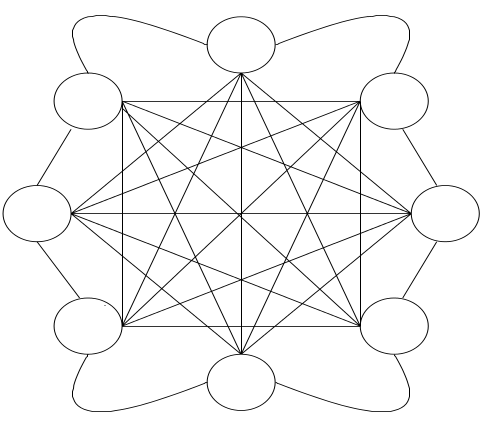
\includegraphics[scale=0.25]{../resources/star}
\end{block}
\end{frame}


\begin{frame}{Topologies III}
\begin{block}{Ring}
Each particle communicates with its $n_\mathcal{N}$ immediate neighbors.
It is employed by \emph{lbest} and takes more time to converge but covers a bigger area in search space.

\centering
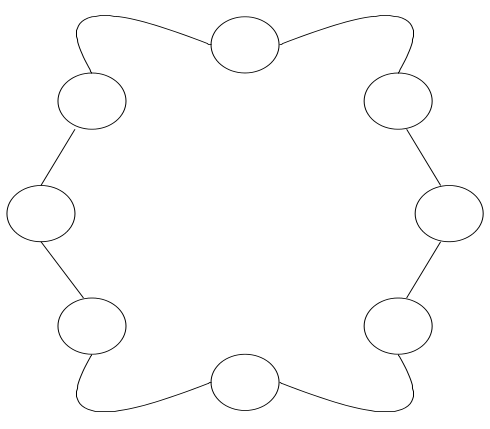
\includegraphics[scale=0.25]{../resources/ring}
\end{block}
\end{frame}

\begin{frame}{Topologies IV}
\begin{block}{Wheel}
Individuals in a neighborhood are isolated from one another.
One particle serves as the focal point, and all information
is communicated through the focal particle.
The focal particle adjusts its position towards the best neighbor. If the new position of the focal particle results in better performance, then the improvement is communicated to all the members of the neighborhood.

\centering
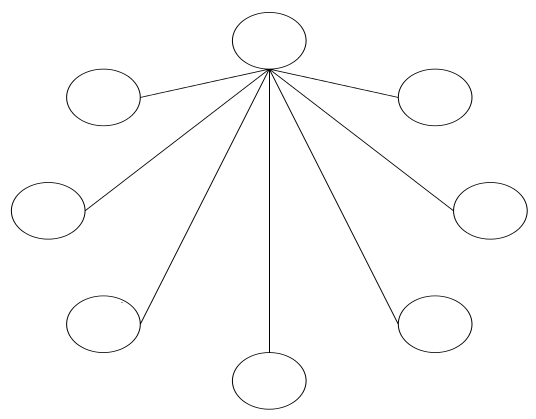
\includegraphics[scale=0.25]{../resources/wheel}
\end{block}
\end{frame}


\begin{frame}{Topologies V}
\begin{block}{Pyramid}
It forms a three-dimensional wire-frame

\centering
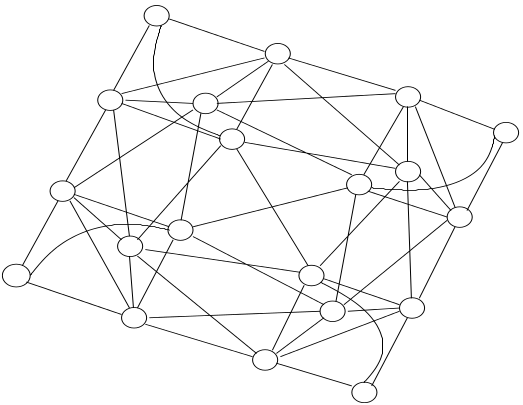
\includegraphics[scale=0.25]{../resources/pyramid}
\end{block}
\end{frame}

\begin{frame}{Topologies VI}
\begin{block}{Four clusters}
Four clusters (or cliques) are formed with two connections between clusters.
Particles within a cluster are connected with five neighbors.

\centering
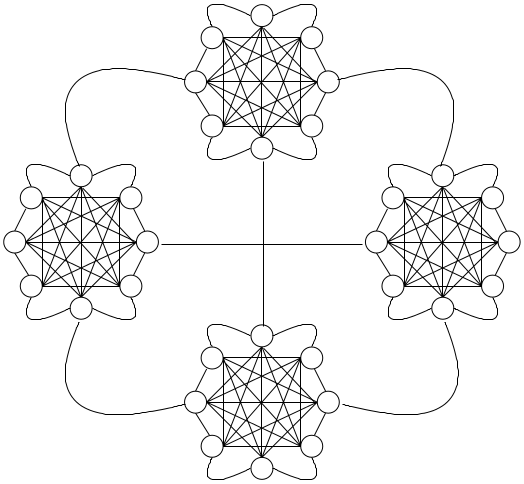
\includegraphics[scale=0.25]{../resources/four-clusters}
\end{block}
\end{frame}

\begin{frame}{Topologies VII}
\begin{block}{Von Neumann}
Particles are connected in a grid structure. 

It has been shown in a number of empirical studies to outperform other social networks in a large number of problems

\centering
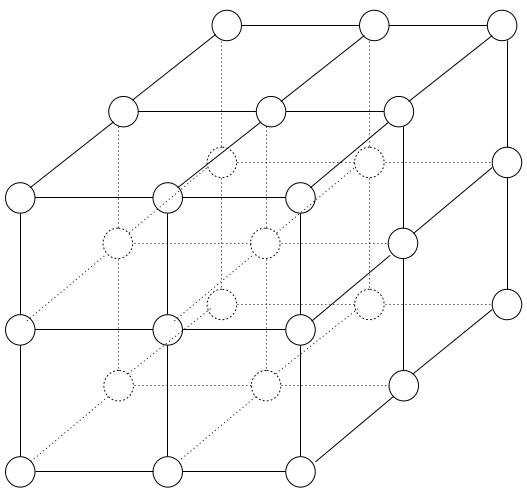
\includegraphics[scale=0.25]{../resources/von-neumann}
\end{block}
\end{frame}

\section{Conclusions}
\begin{frame}{Conclusions}
    \begin{itemize}
    	\item PSO is a technique for optimization.
    	\item It mimics the social behavior of organisms (birds).
    	\item Particles fly toward the optimum, guided by its own knowledge (cognitive) and knoledge of the neighbors (social).
    	\item The core component is the velocity.
    	\item The topology of neighbors affect the communication flow.
    \end{itemize}


\end{frame}
\end{document}